% Asset 25 — the deck's REAL confusion matrix (67 test penguins, logistic
% regression, random_state=42), annotated so it can be read without a
% speaker: rows = truth, columns = prediction, diagonal = right, each
% off-diagonal cell in plain English, row totals (recall) on the right and
% column totals (precision) underneath. Same numbers as the Manim clip.
\documentclass[border=10pt]{standalone}
% Shared preamble for every TikZ diagram in the workshop.
% Included by each asset file with % Shared preamble for every TikZ diagram in the workshop.
% Included by each asset file with % Shared preamble for every TikZ diagram in the workshop.
% Included by each asset file with \input{_preamble}.
%
% Compiled with lualatex so the diagrams use the SAME Inter typeface as the
% slides and the Manim clips. Falls back to the default sans if Inter is not
% installed, so a missing font degrades rather than fails.
\usepackage{iftex}
\ifLuaTeX
  \usepackage{fontspec}
  \IfFontExistsTF{Inter}{%
    \setsansfont{Inter}[
      UprightFont = *-Regular,
      BoldFont    = *-Bold,
      ItalicFont  = *-Italic,
      Extension   = .otf,
    ]%
  }{}
\fi
\renewcommand{\familydefault}{\sfdefault}

\usepackage{amsmath}
\usepackage{tikz}
\usetikzlibrary{positioning,arrows.meta,shapes.geometric,fit,backgrounds,calc,
                matrix,decorations.pathreplacing,patterns}

% --- the shared palette. Blue always means the same thing. ---------------
\definecolor{navy}{HTML}{1B2A4A}     % structure
\definecolor{cblue}{HTML}{2E5CA8}    % class A / train
\definecolor{corange}{HTML}{E07A2C}  % class B / test
\definecolor{cteal}{HTML}{2A9D8F}    % accent
\definecolor{cgray}{HTML}{D9DCE1}    % inactive

\tikzset{
  every picture/.style={line width=0.9pt},
  % a plain labelled container
  box/.style={
    draw=navy, rounded corners=3pt, fill=white,
    minimum width=26mm, minimum height=11mm, align=center,
    text=navy, font=\small
  },
  % a cell in a grid / array / dataframe
  cell/.style={
    draw=navy, fill=white, minimum width=13mm, minimum height=9mm,
    align=center, text=navy, font=\small, inner sep=1pt
  },
  hdr/.style={cell, fill=navy, text=white, font=\scriptsize\bfseries},
  blue/.style={draw=cblue, fill=cblue!12, text=navy},
  orange/.style={draw=corange, fill=corange!14, text=navy},
  teal/.style={draw=cteal, fill=cteal!12, text=navy},
  gray/.style={draw=cgray!140, fill=cgray!35, text=navy},
  % arrows
  arr/.style={-{Stealth[length=3mm,width=2.2mm]}, draw=navy, line width=1pt},
  arrblue/.style={arr, draw=cblue},
  arrorange/.style={arr, draw=corange},
  % text
  capt/.style={text=navy, font=\footnotesize, align=center},
  % fill=white so an annotation that sits on a connector masks it
  % rather than being crossed out by it
  note/.style={text=navy!70, font=\scriptsize\itshape, align=center,
                fill=white, inner sep=2pt},
  ttl/.style={text=navy, font=\bfseries, align=center},
  mono/.style={text=cblue, font=\small\ttfamily},
}
.
%
% Compiled with lualatex so the diagrams use the SAME Inter typeface as the
% slides and the Manim clips. Falls back to the default sans if Inter is not
% installed, so a missing font degrades rather than fails.
\usepackage{iftex}
\ifLuaTeX
  \usepackage{fontspec}
  \IfFontExistsTF{Inter}{%
    \setsansfont{Inter}[
      UprightFont = *-Regular,
      BoldFont    = *-Bold,
      ItalicFont  = *-Italic,
      Extension   = .otf,
    ]%
  }{}
\fi
\renewcommand{\familydefault}{\sfdefault}

\usepackage{amsmath}
\usepackage{tikz}
\usetikzlibrary{positioning,arrows.meta,shapes.geometric,fit,backgrounds,calc,
                matrix,decorations.pathreplacing,patterns}

% --- the shared palette. Blue always means the same thing. ---------------
\definecolor{navy}{HTML}{1B2A4A}     % structure
\definecolor{cblue}{HTML}{2E5CA8}    % class A / train
\definecolor{corange}{HTML}{E07A2C}  % class B / test
\definecolor{cteal}{HTML}{2A9D8F}    % accent
\definecolor{cgray}{HTML}{D9DCE1}    % inactive

\tikzset{
  every picture/.style={line width=0.9pt},
  % a plain labelled container
  box/.style={
    draw=navy, rounded corners=3pt, fill=white,
    minimum width=26mm, minimum height=11mm, align=center,
    text=navy, font=\small
  },
  % a cell in a grid / array / dataframe
  cell/.style={
    draw=navy, fill=white, minimum width=13mm, minimum height=9mm,
    align=center, text=navy, font=\small, inner sep=1pt
  },
  hdr/.style={cell, fill=navy, text=white, font=\scriptsize\bfseries},
  blue/.style={draw=cblue, fill=cblue!12, text=navy},
  orange/.style={draw=corange, fill=corange!14, text=navy},
  teal/.style={draw=cteal, fill=cteal!12, text=navy},
  gray/.style={draw=cgray!140, fill=cgray!35, text=navy},
  % arrows
  arr/.style={-{Stealth[length=3mm,width=2.2mm]}, draw=navy, line width=1pt},
  arrblue/.style={arr, draw=cblue},
  arrorange/.style={arr, draw=corange},
  % text
  capt/.style={text=navy, font=\footnotesize, align=center},
  % fill=white so an annotation that sits on a connector masks it
  % rather than being crossed out by it
  note/.style={text=navy!70, font=\scriptsize\itshape, align=center,
                fill=white, inner sep=2pt},
  ttl/.style={text=navy, font=\bfseries, align=center},
  mono/.style={text=cblue, font=\small\ttfamily},
}
.
%
% Compiled with lualatex so the diagrams use the SAME Inter typeface as the
% slides and the Manim clips. Falls back to the default sans if Inter is not
% installed, so a missing font degrades rather than fails.
\usepackage{iftex}
\ifLuaTeX
  \usepackage{fontspec}
  \IfFontExistsTF{Inter}{%
    \setsansfont{Inter}[
      UprightFont = *-Regular,
      BoldFont    = *-Bold,
      ItalicFont  = *-Italic,
      Extension   = .otf,
    ]%
  }{}
\fi
\renewcommand{\familydefault}{\sfdefault}

\usepackage{amsmath}
\usepackage{tikz}
\usetikzlibrary{positioning,arrows.meta,shapes.geometric,fit,backgrounds,calc,
                matrix,decorations.pathreplacing,patterns}

% --- the shared palette. Blue always means the same thing. ---------------
\definecolor{navy}{HTML}{1B2A4A}     % structure
\definecolor{cblue}{HTML}{2E5CA8}    % class A / train
\definecolor{corange}{HTML}{E07A2C}  % class B / test
\definecolor{cteal}{HTML}{2A9D8F}    % accent
\definecolor{cgray}{HTML}{D9DCE1}    % inactive

\tikzset{
  every picture/.style={line width=0.9pt},
  % a plain labelled container
  box/.style={
    draw=navy, rounded corners=3pt, fill=white,
    minimum width=26mm, minimum height=11mm, align=center,
    text=navy, font=\small
  },
  % a cell in a grid / array / dataframe
  cell/.style={
    draw=navy, fill=white, minimum width=13mm, minimum height=9mm,
    align=center, text=navy, font=\small, inner sep=1pt
  },
  hdr/.style={cell, fill=navy, text=white, font=\scriptsize\bfseries},
  blue/.style={draw=cblue, fill=cblue!12, text=navy},
  orange/.style={draw=corange, fill=corange!14, text=navy},
  teal/.style={draw=cteal, fill=cteal!12, text=navy},
  gray/.style={draw=cgray!140, fill=cgray!35, text=navy},
  % arrows
  arr/.style={-{Stealth[length=3mm,width=2.2mm]}, draw=navy, line width=1pt},
  arrblue/.style={arr, draw=cblue},
  arrorange/.style={arr, draw=corange},
  % text
  capt/.style={text=navy, font=\footnotesize, align=center},
  % fill=white so an annotation that sits on a connector masks it
  % rather than being crossed out by it
  note/.style={text=navy!70, font=\scriptsize\itshape, align=center,
                fill=white, inner sep=2pt},
  ttl/.style={text=navy, font=\bfseries, align=center},
  mono/.style={text=cblue, font=\small\ttfamily},
}

\begin{document}
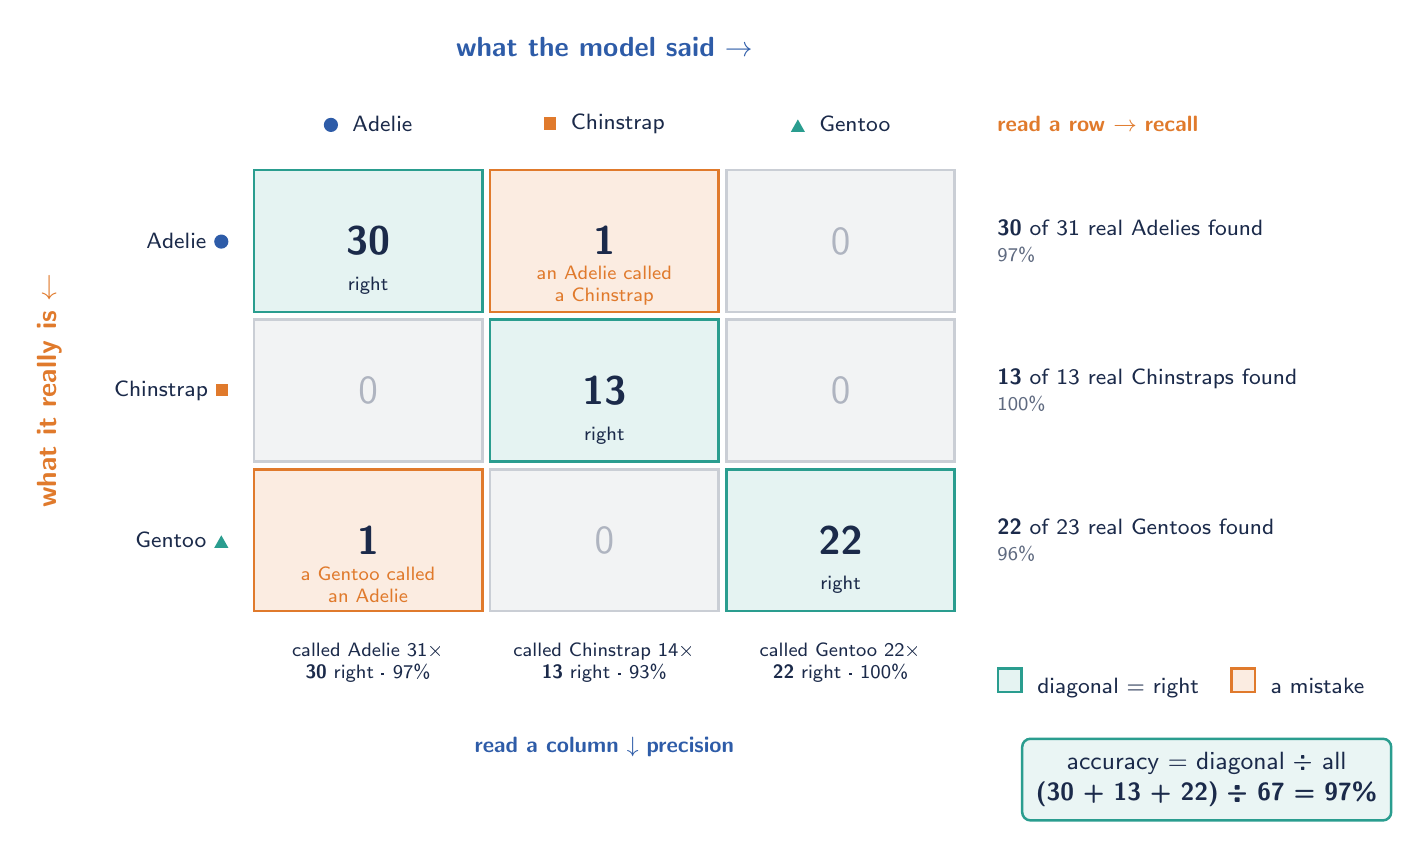
\begin{tikzpicture}[x=30mm, y=19mm,
  ok/.style={cell, teal, minimum width=29mm, minimum height=18mm, font=\Large\bfseries},
  bad/.style={cell, orange, minimum width=29mm, minimum height=18mm, font=\Large\bfseries},
  nil/.style={cell, gray, minimum width=29mm, minimum height=18mm, font=\Large, text=navy!35},
  sub/.style={font=\scriptsize, text=navy, align=center},
  side/.style={font=\footnotesize, text=navy, align=left, anchor=west},
]

% ---- column headers: what the model said
\node[ttl, text=cblue] at (2,3.3) {what the model \textbf{said} $\rightarrow$};
\node[capt] at (1,2.78) {\tikz\fill[cblue] (0,0) circle (0.9mm);\; Adelie};
\node[capt] at (2,2.78) {\tikz\fill[corange] (0,0) rectangle (1.6mm,1.6mm);\; Chinstrap};
\node[capt] at (3,2.78) {\tikz\fill[cteal] (0,0) -- (1.8mm,0) -- (0.9mm,1.6mm) -- cycle;\; Gentoo};

% ---- row headers: what it really is
\node[ttl, text=corange, rotate=90] at (-0.35,1) {what it \textbf{really} is $\leftarrow$};
\node[capt, anchor=east] at (0.45,2) {Adelie \tikz\fill[cblue] (0,0) circle (0.9mm);};
\node[capt, anchor=east] at (0.45,1) {Chinstrap \tikz\fill[corange] (0,0) rectangle (1.6mm,1.6mm);};
\node[capt, anchor=east] at (0.45,0) {Gentoo \tikz\fill[cteal] (0,0) -- (1.8mm,0) -- (0.9mm,1.6mm) -- cycle;};

% ---- the nine cells (row = truth, column = prediction)
\node[ok]  (aa) at (1,2) {30};
\node[bad] (ac) at (2,2) {1};
\node[nil] at (3,2) {0};
\node[nil] at (1,1) {0};
\node[ok]  (cc) at (2,1) {13};
\node[nil] at (3,1) {0};
\node[bad] (ga) at (1,0) {1};
\node[nil] at (2,0) {0};
\node[ok]  (gg) at (3,0) {22};

% plain-English captions inside the interesting cells
\node[sub] at ($(aa)+(0,-0.3)$) {right};
\node[sub] at ($(cc)+(0,-0.3)$) {right};
\node[sub] at ($(gg)+(0,-0.3)$) {right};
\node[sub, text=corange] at ($(ac)+(0,-0.3)$) {an Adelie called\\a Chinstrap};
\node[sub, text=corange] at ($(ga)+(0,-0.3)$) {a Gentoo called\\an Adelie};

% legend for the two colours (the diagonal is the teal cells)
\node[capt, anchor=west, font=\footnotesize] at (3.62,-0.95)
     {\tikz\draw[cteal, fill=cteal!12] (0,0) rectangle (3mm,3mm);\; diagonal = right \quad
      \tikz\draw[corange, fill=corange!14] (0,0) rectangle (3mm,3mm);\; a mistake};

% ---- row totals: of the real ones, how many found? (recall)
\node[side] at (3.62,2.0) {\textbf{30} of 31 real Adelies found\\\scriptsize\color{navy!70} 97\%};
\node[side] at (3.62,1.0) {\textbf{13} of 13 real Chinstraps found\\\scriptsize\color{navy!70} 100\%};
\node[side] at (3.62,0.0) {\textbf{22} of 23 real Gentoos found\\\scriptsize\color{navy!70} 96\%};
\node[capt, text=corange, font=\footnotesize\bfseries, anchor=west] at (3.62,2.78) {read a row $\rightarrow$ \textsl{recall}};

% ---- column totals: of those it named, how many were right? (precision)
\node[sub] at (1,-0.82) {called Adelie 31×\\\textbf{30} right · 97\%};
\node[sub] at (2,-0.82) {called Chinstrap 14×\\\textbf{13} right · 93\%};
\node[sub] at (3,-0.82) {called Gentoo 22×\\\textbf{22} right · 100\%};
\node[capt, text=cblue, font=\footnotesize\bfseries] at (2,-1.38) {read a column $\downarrow$ \textsl{precision}};

% ---- accuracy
\node[draw=cteal, fill=cteal!10, rounded corners=3pt, inner sep=5pt, text=navy,
      font=\small, align=center] at (4.55,-1.6)
     {accuracy = diagonal ÷ all\\\textbf{(30 + 13 + 22) ÷ 67 = 97\%}};

\end{tikzpicture}
\end{document}
